\documentclass[screen, aspectratio=169]{beamer}
\usepackage[T1]{fontenc}
\usepackage[utf8]{inputenc}

% Use the NTNU-temaet for beamer 
% \usetheme[style=ntnu|simple|vertical|horizontal, 
%     language=bm|nn|en, 
%     smalltitle, 
%     city=all|trondheim|alesund|gjovik]{ntnu2017}
\usetheme[style=ntnu, language=en, smalltitle]{ntnu2017}

\usepackage[english]{babel}
\usepackage[style=numeric,backend=biber,natbib=false,sorting=none]{biblatex}

\title[PCW-d1]{Physical Computing Workshop\\2nd edition}
\subtitle{Introduction}
\author[A. Xamb{\'o}]{Anna Xamb{\'o}}
\institute[NTNU]{Department of Music, NTNU}
\date{15 October 2019}
%\date{} % To have an empty date

\addbibresource{../pcw.bib} % Add bibliography database

% Set the reference style to numeric.
% See here: http://tex.stackexchange.com/questions/68080/beamer-bibliography-icon
\setbeamertemplate{bibliography item}[text] 

% Set bibliography fonts to a small size.
\renewcommand*{\bibfont}{\footnotesize}

\begin{document}

\begin{frame}
  \titlepage
\end{frame}

% Alternatively, special title page command to get a different background
% \ntnutitlepage


\begin{frame}
\frametitle{Workshop Design Criteria}
\begin{itemize}
\item Facilitate a hands-on workshop with affordable and DIY technologies (e.g. contact microphones, raw loudspeakers, Bela boards, Pd software).
\item Explore individually and in group the fundamental concepts behind physical computing (e.g. tinkering, programming, making).
\item Promote a sharing culture of code and discoveries (e.g. writing reflective blog posts, sharing code repositories).
\item Contextualize the workshop to the broader context of interactive systems for music performance at both theoretical and practical levels (e.g. readings, practices).
\end{itemize}
\end{frame}
%
\begin{frame}
\frametitle{What is the Workshop About?}
\begin{itemize}
\item An intense 4-day workshop where you will explore physical computing and interactive systems.
\item For the first three days, there will be a theme with paced exercises.
\item At the beginning of each session there will be a warm-up activity related to the topic.
\item At the end of each session there will be a network music performance to showcase the own-built prototype.
\item On the last day, there will be a mini-hackathon where you will develop an interactive system for music performance mixing technologies and techniques learned throughout the workshop.
\item Each team will write a blog post about the challenges and opportunities of their own-built prototype.
\end{itemize}
\end{frame}
%
\begin{frame}
\frametitle{General Learning Outcomes}
\begin{itemize}
\item Develop skills of computational thinking and programming.
\item Explore how to create a prototype of an interactive system for music performance with low-tech technologies.
\item Discover iterative design and the possibilities of network music by performing with own-built prototypes.
\item Develop critical thinking skills applied to reflection on artistic practice and instrument building.
\end{itemize}
\end{frame}
%
\begin{frame}
\frametitle{General Approach}
\begin{itemize}
\item This workshop should be seen as a starting point to get interest with physical computing applied to interactive music systems.
\item It has been designed to be low tech, that is, using open source or consumer affordable gadgets.
\item It has been designed to be participatory and playful.
\end{itemize}
\end{frame}
%
\begin{frame}
\frametitle{What it is not}
\begin{itemize}
\item An in-depth tutorial of a particular technology.
\item A technical course: just enough to build things!
\item A course about soldering.
\end{itemize}
However... related resources will be provided.
\end{frame}
%
\begin{frame}
\frametitle{Grading}
\begin{itemize}
\item The Physical Computing workshop is evaluated with a Pass/Fail grade.
\item Attendance is required to pass because the workshop consist of practical group work, collective participation and discussion. Active engagement in the tasks at hand is also required to pass. 
\item You will be expected to participate in the daily performance.
\item You will be expected to contribute to the two blogposts of the workshops.
\end{itemize}
\end{frame}
%
\begin{frame}
\frametitle{Previous Knowledge / Preparation}
\begin{itemize}
\item No previous knowledge is required. This workshop is designed to be a standalone workshop. The preparation material is described in the description of each session on Canvas.
\item Every day you should check if there is a list of items that need to be brought to class.
\item Every day you should check whether there are suggested readings that might be discussed at the beginning of the class.
\end{itemize}
\end{frame}
%
\begin{frame}
\frametitle{Recommended General Readings}
\begin{figure}
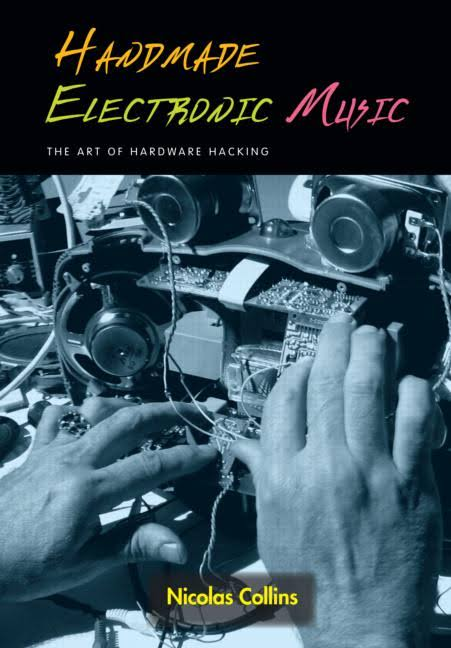
\includegraphics[scale=0.2]{img/HEM-collins-book.jpg}
\end{figure}
\begin{itemize}
\item The book \emph{Handmade Electronic Music} by Nicolas Collins~\cite{Collins.2006.handmadebook}.
\item ... and in general all the videos related to Collins' book:\\
\url{https://www.nicolascollins.com/video/}
\end{itemize}
\end{frame}
%
\begin{frame}
\frametitle{Recommended General Readings}
\begin{figure}
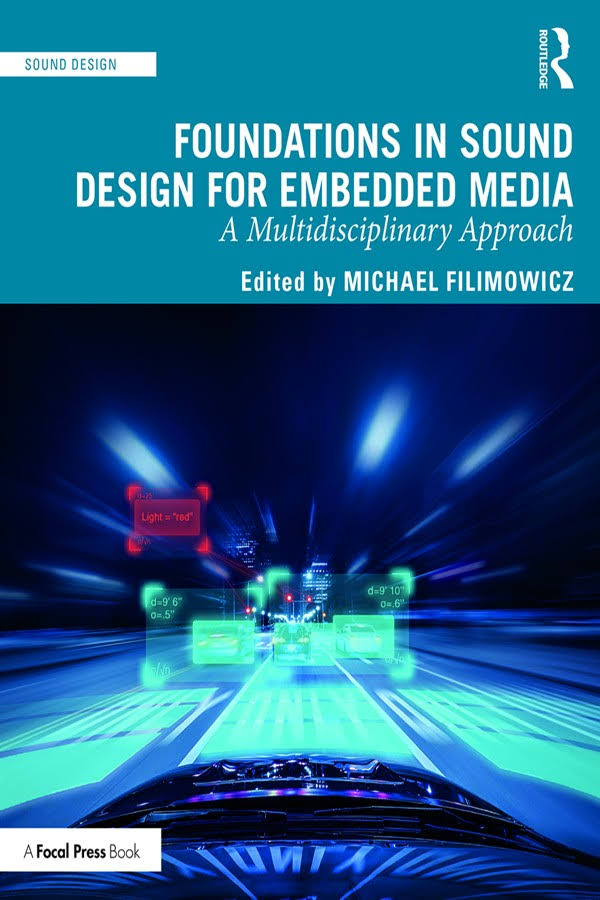
\includegraphics[scale=0.15]{img/Routledge-embedded-media.jpg}
\end{figure}
\begin{itemize}
\item The book \emph{Foundations in Sound Design for Embedded Media: A Multidisciplinary Approach} by Michael Filimowicz (ed)~\cite{Filimowicz.2019}.
\end{itemize}
\end{frame}
%
\begin{frame}
\frametitle{Recommended General Readings}
\begin{figure}
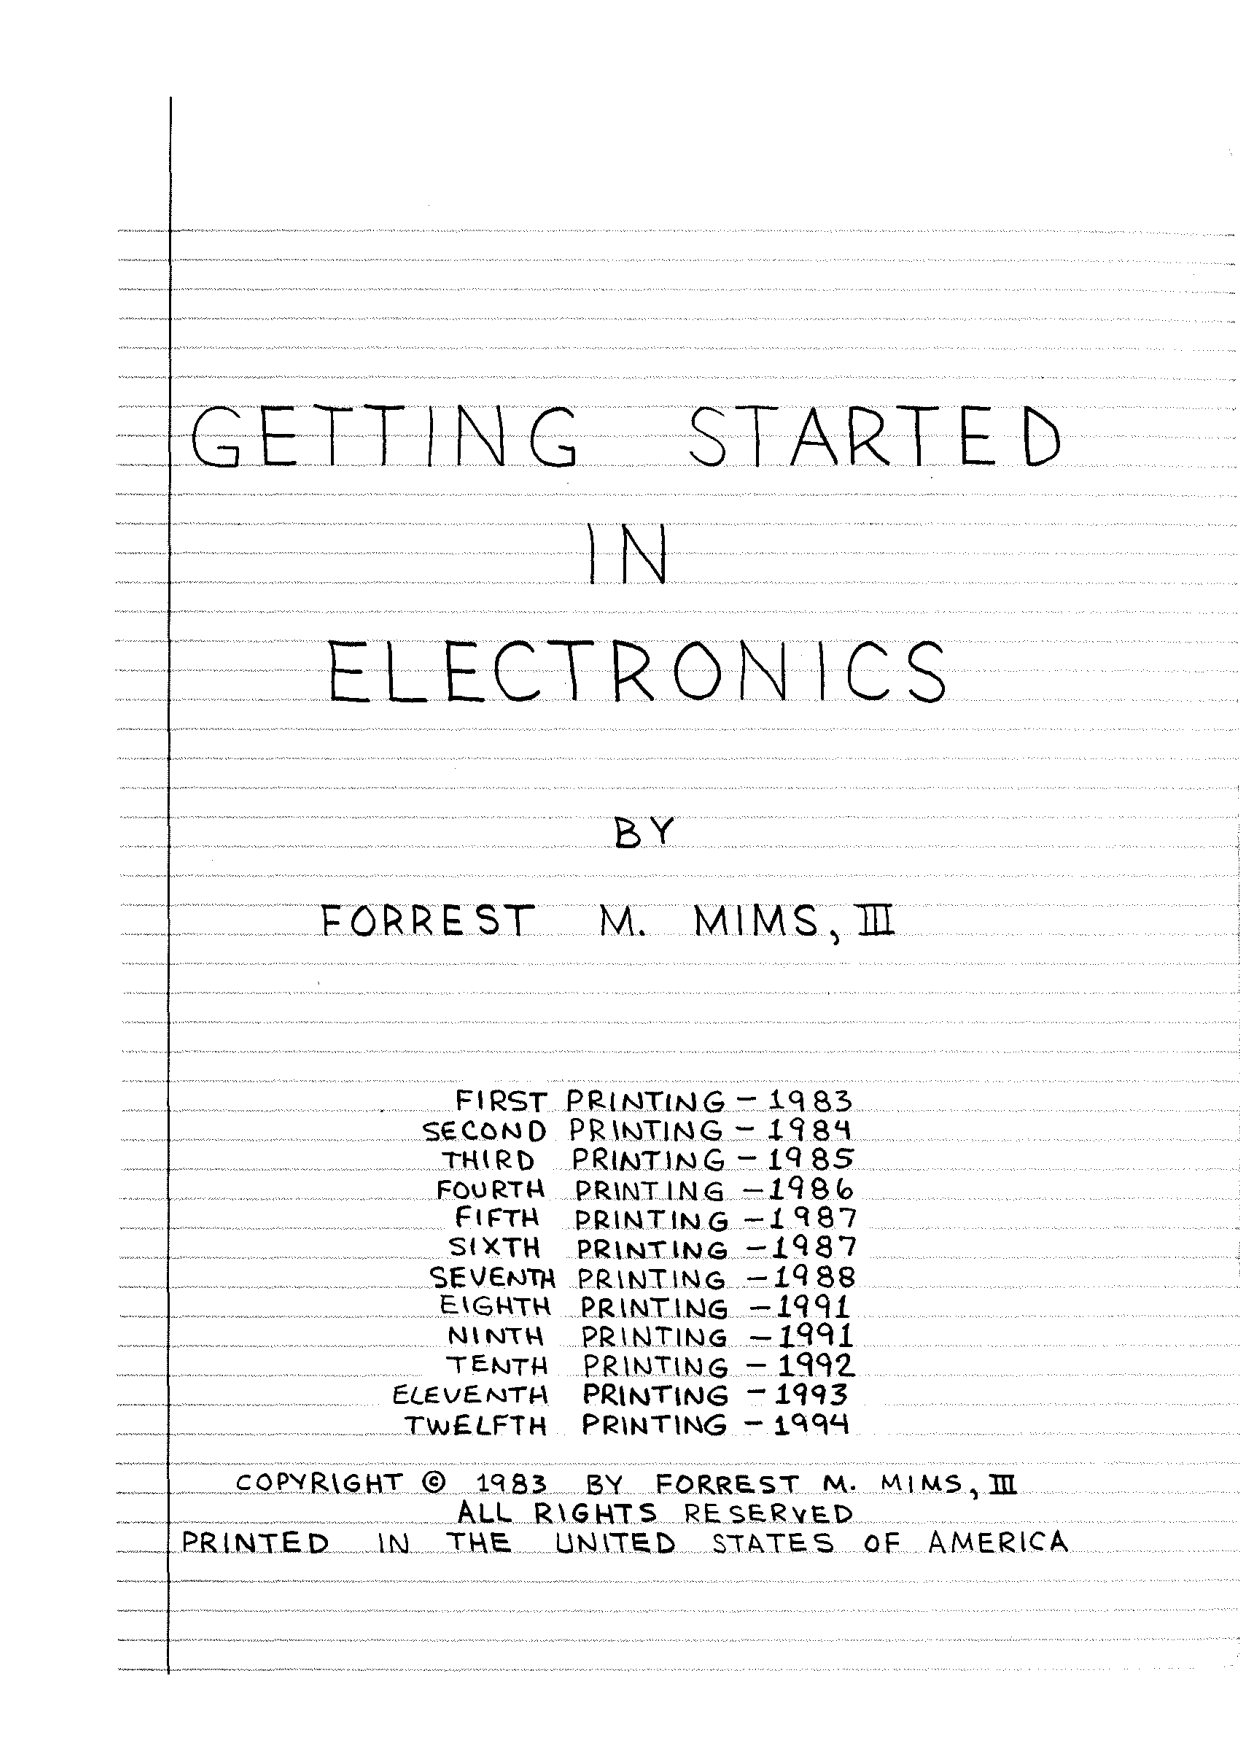
\includegraphics[scale=0.2]{img/gettingstartedelectronics-book.pdf}
\end{figure}
\begin{itemize}
\item The book \emph{Getting Started in Electronics} by Forrest Mims~\cite{Mims.1983.radioshack}.
\end{itemize}
\end{frame}
%
\begin{frame}
\frametitle{Tips}
\begin{itemize}
\item Divide and conquer (Dijkstra).
\item It can take up to 10 years to become an expert programmer. Focus on learning programming strategies instead of knowledge \cite{Robins.2003.learning}.
\item Enjoy the beauty of the ephemeral.
\end{itemize}
\end{frame}
%
\begin{frame}
  \frametitle{References}
  \printbibliography
\end{frame}
%
\end{document}
